% Worked example (appendix): TikZ, same style as the teaser. Values from out/paper/data/fig4_worked_example.json
% (case eval12@01cfbb1e713f-13e92662d1, database insider, arithmetic depth 1, step depth 3) and library/examples.jsonl (bird_pairs:b034).
% Shared setup for the diagrams (teaser, pipeline, worked). Built with XeLaTeX so that all text is Arial, in black.
% Sizes match the paper's acmart sigconf sizes (\footnotesize 7 pt); the smallest text is 6 pt.
\documentclass[border=0.5pt]{standalone}
\usepackage{fontspec}
\setmainfont{Arial}\setsansfont{Arial}\setmonofont{Menlo}[Scale=MatchLowercase]
\usepackage{unicode-math}\setmathfont{FiraMath-Regular.otf}
\usepackage{booktabs}
\usepackage{tikz}
\usetikzlibrary{arrows.meta,calc,positioning,fit,backgrounds,shapes.geometric}
\renewcommand\large{\fontsize{10}{12}\selectfont}
\renewcommand\small{\fontsize{8}{10}\selectfont}
\renewcommand\footnotesize{\fontsize{7}{8.4}\selectfont}
\renewcommand\scriptsize{\fontsize{6.5}{7.6}\selectfont}
\renewcommand\tiny{\fontsize{6}{7}\selectfont}
\newcommand{\nohyph}{\hyphenpenalty=10000\exhyphenpenalty=10000\relax}
\newcommand{\sql}[1]{\texttt{#1}}
% the edited SQL clause, highlighted as in AMBROSIA and the test-suite paper; plain check and cross marks
\newcommand{\hl}[2]{{\setlength{\fboxsep}{0.7pt}\colorbox{#1f}{\vphantom{Ay}\texttt{#2}}}}
\newfontfamily\markfont{Arial Unicode MS}\newcommand{\yes}{{\markfont ✓}}\newcommand{\no}{{\markfont ✗}}
% math letters in Arial italic; the open-request circle is drawn; only the arrow comes from Fira Math
\newcommand{\vq}[1]{\textit{q}\textsubscript{#1}}\newcommand{\vp}[1]{\textit{p}\textsubscript{#1}}\newcommand{\vo}{\mbox{\textit{q}\hspace{0.3pt}\raisebox{-0.25ex}{\tikz[baseline=0pt]\draw[line width=0.45pt] (0,1.1pt) circle (1.1pt);}}}
% box lines: A (blue) and B (orange) as in the data figures; neutral lines grey. Text is always black.
% colors as in AMBROSIA's and AmbiQT's diagrams (draw.io palette): interpretation A blue, interpretation B orange, code blocks light gray
\definecolor{sbA}{HTML}{6C8EBF}\definecolor{sbB}{HTML}{D79B00}\definecolor{sbAf}{HTML}{DAE8FC}\definecolor{sbBf}{HTML}{FFE6CC}\definecolor{sbline}{HTML}{4D4D4D}
\definecolor{sbfill}{HTML}{F5F5F5}

\begin{document}
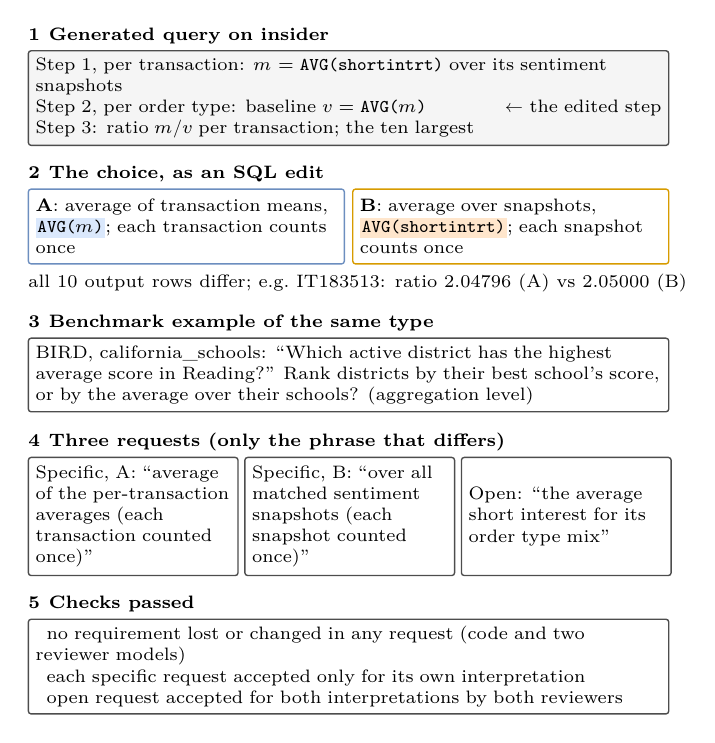
\begin{tikzpicture}[x=1cm, y=1cm, font=\scriptsize, >=Stealth, line width=0.5pt,
  bx/.style={execute at begin node=\nohyph, draw=sbline, rounded corners=1pt, inner sep=2.6pt, align=left, text width=7.95cm, anchor=north west},
  hd/.style={font=\scriptsize\bfseries, text=black, anchor=north west, inner sep=0pt},
  arr/.style={->, draw=sbline}]
% ---- 1 the generated query
\node[hd] (h1) at (0,0) {1\enspace Generated query on {insider}};
\node[bx, fill=sbfill] (q) at ([yshift=-2pt]h1.south west) {%
Step 1, per transaction: $m$ = \sql{AVG(shortintrt)} over its sentiment snapshots\\
Step 2, per order type: baseline $v$ = {\sql{AVG($m$)}} \hfill {$\leftarrow$ the edited step}\\
Step 3: ratio $m/v$ per transaction; the ten largest};
% ---- 2 the decision and its execution
\node[hd] (h2) at ([yshift=-7pt]q.south west) {2\enspace The choice, as an SQL edit};
\node[bx, draw=sbA, text width=3.83cm, minimum height=0.95cm] (a) at ([yshift=-2pt]h2.south west) {\textbf{A}: average of transaction means, \hl{sbA}{AVG($m$)}; each transaction counts once};
\node[bx, draw=sbB, text width=3.83cm, minimum height=0.95cm] (b) at ([xshift=4.12cm]a.north west) {\textbf{B}: average over snapshots, \hl{sbB}{AVG(shortintrt)}; each snapshot counts once};
\node[anchor=north west, inner sep=0pt] (w) at ([yshift=-3pt]a.south west) {\scriptsize all 10 output rows differ; e.g.\ {IT183513}: ratio {2.04796} (A) vs {2.05000} (B)};
% ---- 3 library example
\node[hd] (h3) at ([yshift=-8pt]w.south west) {3\enspace Benchmark example of the same type};
\node[bx] (l) at ([yshift=-2pt]h3.south west) {BIRD, {california\_schools}: ``Which active district has the highest average score in Reading?''
Rank districts by their best school's score, or by the average over their schools? (aggregation level)};
% ---- 4 three wordings
\node[hd] (h4) at ([yshift=-7pt]l.south west) {4\enspace Three requests (only the phrase that differs)};
\node[bx, text width=2.48cm, minimum height=1.5cm] (qa) at ([yshift=-2pt]h4.south west) {Specific, A: ``average of the per-transaction averages (each transaction counted once)''};
\node[bx, text width=2.48cm, minimum height=1.5cm] (qb) at ([xshift=2.75cm]qa.north west) {Specific, B: ``over all matched sentiment snapshots (each snapshot counted once)''};
\node[bx, text width=2.48cm, minimum height=1.5cm] (qo) at ([xshift=5.5cm]qa.north west) {Open: ``the average short interest for its order type mix''};
% ---- 5 checks
\node[hd] (h5) at ([yshift=-7pt]qa.south west) {5\enspace Checks passed};
\node[bx] (c) at ([yshift=-2pt]h5.south west) {%
\yes\ no requirement lost or changed in any request (code and two reviewer models)\\
\yes\ each specific request accepted only for its own interpretation\\
\yes\ open request accepted for both interpretations by both reviewers};
\end{tikzpicture}
\end{document}
